\documentclass[]{article}
\usepackage{lmodern}
\usepackage{amssymb,amsmath}
\usepackage{ifxetex,ifluatex}
\usepackage{fixltx2e} % provides \textsubscript
\ifnum 0\ifxetex 1\fi\ifluatex 1\fi=0 % if pdftex
  \usepackage[T1]{fontenc}
  \usepackage[utf8]{inputenc}
\else % if luatex or xelatex
  \ifxetex
    \usepackage{mathspec}
  \else
    \usepackage{fontspec}
  \fi
  \defaultfontfeatures{Ligatures=TeX,Scale=MatchLowercase}
\fi
% use upquote if available, for straight quotes in verbatim environments
\IfFileExists{upquote.sty}{\usepackage{upquote}}{}
% use microtype if available
\IfFileExists{microtype.sty}{%
\usepackage{microtype}
\UseMicrotypeSet[protrusion]{basicmath} % disable protrusion for tt fonts
}{}
\usepackage[margin=1in]{geometry}
\usepackage{hyperref}
\hypersetup{unicode=true,
            pdftitle={A Robust Approach to Automatic Groove Identification in 3D Bullet Land Scans},
            pdfauthor={Kiegan Rice, M.Sc., Heike Hofmann, Ph.D., Ulrike Genschel, Ph.D.},
            pdfborder={0 0 0},
            breaklinks=true}
\urlstyle{same}  % don't use monospace font for urls
\usepackage{natbib}
\bibliographystyle{plainnat}
\usepackage{graphicx,grffile}
\makeatletter
\def\maxwidth{\ifdim\Gin@nat@width>\linewidth\linewidth\else\Gin@nat@width\fi}
\def\maxheight{\ifdim\Gin@nat@height>\textheight\textheight\else\Gin@nat@height\fi}
\makeatother
% Scale images if necessary, so that they will not overflow the page
% margins by default, and it is still possible to overwrite the defaults
% using explicit options in \includegraphics[width, height, ...]{}
\setkeys{Gin}{width=\maxwidth,height=\maxheight,keepaspectratio}
\IfFileExists{parskip.sty}{%
\usepackage{parskip}
}{% else
\setlength{\parindent}{0pt}
\setlength{\parskip}{6pt plus 2pt minus 1pt}
}
\setlength{\emergencystretch}{3em}  % prevent overfull lines
\providecommand{\tightlist}{%
  \setlength{\itemsep}{0pt}\setlength{\parskip}{0pt}}
\setcounter{secnumdepth}{5}
% Redefines (sub)paragraphs to behave more like sections
\ifx\paragraph\undefined\else
\let\oldparagraph\paragraph
\renewcommand{\paragraph}[1]{\oldparagraph{#1}\mbox{}}
\fi
\ifx\subparagraph\undefined\else
\let\oldsubparagraph\subparagraph
\renewcommand{\subparagraph}[1]{\oldsubparagraph{#1}\mbox{}}
\fi

%%% Use protect on footnotes to avoid problems with footnotes in titles
\let\rmarkdownfootnote\footnote%
\def\footnote{\protect\rmarkdownfootnote}

%%% Change title format to be more compact
\usepackage{titling}

% Create subtitle command for use in maketitle
\newcommand{\subtitle}[1]{
  \posttitle{
    \begin{center}\large#1\end{center}
    }
}

\setlength{\droptitle}{-2em}

  \title{A Robust Approach to Automatic Groove Identification in 3D Bullet Land
Scans}
    \pretitle{\vspace{\droptitle}\centering\huge}
  \posttitle{\par}
    \author{Kiegan Rice, M.Sc., Heike Hofmann, Ph.D., Ulrike Genschel, Ph.D.}
    \preauthor{\centering\large\emph}
  \postauthor{\par}
    \date{}
    \predate{}\postdate{}
  

\begin{document}
\maketitle
\begin{abstract}
Forensic firearms examiners analyze bullets through a process of visual
feature comparison to determine whether two bullets originate from the
same source or different sources. Striation marks found on land engraved
areas (LEAs) provide evidence to address this same source-different
source problem. Advances in technology have led to an increase in
research focused on applying image-analysis algorithms to the automated,
quantitative analysis of bullet evidence. One prominent example is an
algorithm developed by \citep{Hare1} based on 3D imaging data of LEAs.
This algorithm relies on removal of the overall curve of the bullet to
obtain what \citep{Hare1} refer to as a ``signature''. Cross-correlation
functions, consecutive matching striae, consecutive non-matching striae
and other features are then calculated based on pairwise comparisons of
these signatures. The currently established best practice for collection
of 3D images of bullet LEAs requires capturing portions of the
neighboring groove engraved areas (GEAs). Dealing with LEA and GEA data
separately is crucial to aim for high accuracy and precision in
subsequent feature calculations. However, standard statistical modeling
techniques fall short when applied to the atypical structure of 3D
bullet data, often failing to adequately separate LEA and GEA data. The
following work describes a better solution to this pre-processing
problem based on robust statistical models.
\end{abstract}

TODO:

\section{Background}

Forensic firearms examiners analyze bullets through a process of visual
feature comparison. The main objective of visual feature comparison is
to determine whether two patterns were generated by the same object.
This problem is known in forensic science as the \emph{same
source-different source problem}. In forensic firearms analysis, the
same source-different source problem is focused on whether two bullets
were propelled through the same gun barrel.

Striation marks, which are engraved on the surface of a bullet through
contact with the rifling of a gun barrel, provide evidence to address
the same source-different source problem. Alternating sections of the
bullet that make the closest contact with the barrel are called land
engraved areas (LEAs). A guiding principle in forensic firearms analysis
is that two bullets fired through the same barrel will bear more similar
striation marks on their LEAs than two bullets fired from different
barrels.

Evidence is examined using a comparison microscope: two bullets in
question are placed under the microscope and firearms examiners make a
decision according to the AFTE Theory of Identification \citep{AFTE}.

In the last several decades, advances in technology have led to an
increase in research focused on developing image-analysis algorithms to
complete automated, quantitative analyses of bullet evidence. The main
technological development that has created a pathway for image-analysis
techniques is the introduction of high resolution 3D scanning technology
to the field of forensic science
\citep[e.g.~][]{DeKinder1, DeKinder2, Bachrach1}. These 3D data have
since been used in the development of several methods of varying
complexity for automated comparison of land engraved areas
\citep[e.g.~][]{Ma1, Chu1, Chu2, Hare1}.

\citet{Hare1} proposes a matching algorithm based on 3D imaging data of
LEAs. Horizontal slices of the 3D images, called profiles, provide a
detailed representation of striae impressed on the surface at a
horizontal cross-section of each LEA.

Removal of the overall curve of the bullet -- the global structure
captured in the 3D scanning process -- transforms these profiles into to
what \citet{Hare1} refer to as signatures. For a land-to-land
comparison, features such as cross-correlation function, consecutive
matching striae \citep[see][]{Biasotti}, and consecutive non-matching
striae are calculated based on two aligned signatures. These calculated
features are the information used in a random forest model to assess the
similarity of the corresponding pair of signatures.

Extraction of the aforementioned features depends on the step which
translates a profile to a signature: the removal of the global
structure. This step is complicated by the 3D data collection process.

While there is not yet an established standard operating procedure, the
currently established best practice for collection of 3D images of
bullet LEAs requires that scanning across the object must begin and end
in the neighboring groove engraved areas (GEAs) as shown in
\autoref{fig:LEA}. However, this practice introduces a challenging data
structure. The presence of extraneous GEA data dictates the most
significant step in data pre-processing: correctly identifying between
data from LEAs and GEAs.

Dealing with these two areas separately is crucial to aim for high
accuracy and precision in subsequent processing steps. Removal of data
from groove engraved areas is necessary to properly calculate features
used in automated comparisons. In order to distinguish between these
areas, we aim to identify ``shoulder locations'', the locations at which
the LEA ends and the GEAs begin.

\section{Data Source}

The data used in this paper consist of high resolution 3D scans of
bullet land engraved areas (LEAs). The scanned bullets come from Hamby
Set 44 \citep{Hamby}. Each Hamby set consists of 35 bullets fired from
10 consecutively rifled Ruger P85 barrels. There are two known bullets
for each of the ten barrels, as well as 15 additional questioned bullets
in each set. Each fired bullet in Hamby Set 44 has 6 LEAs; every LEA was
scanned for each of the 35 bullets, producing data for 210 individual
lands. Two lands -- Barrel 9, Bullet 2, Land 3 and Unknowns, Bullet L,
Land 5 -- were removed from consideration due to ``tank rash''. Tank
rash results from a bullet striking the bottom of a water recovery tank
after exiting the barrel, thereby creating marks on the land that are
not due to the contact with the barrel.

The 3D scans of Hamby Set 44 were captured with a Sensofar Confocal
light microscope at 20x magnification resulting in a resolution of 0.645
microns per pixel. These LEAs were scanned at Iowa State University's
High Resolution Microscopy Facility, and the scans are stored in 3D
format as x3p files, conforming to the ISO5436-2 standard
\citep{ISO5436}. A visualization of the data gathered for a single LEA
is seen in \autoref{fig:LEA}. Physically, each land is approximately 2
millimeters in width; as such, data structures for a single LEA can
contain more than 3 million individual data points.

\begin{figure}
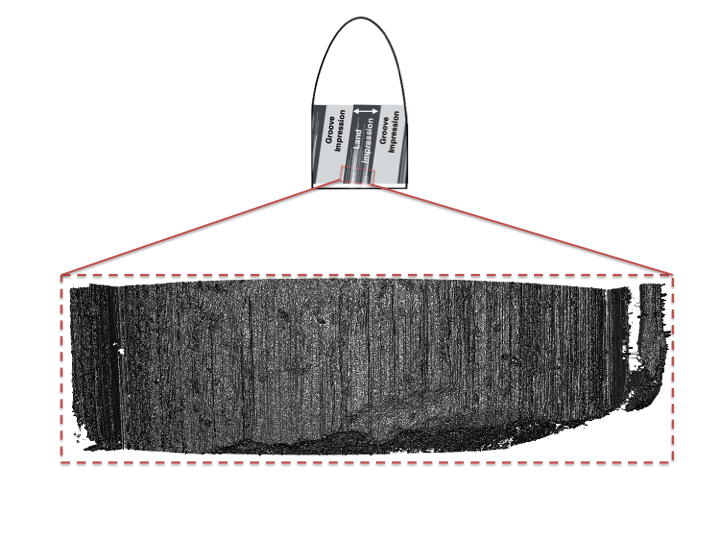
\includegraphics[width=\textwidth]{./images/3d_plot_top_context_breakoff} \caption{\label{LEA}Visualization of 3D data collected through high resolution scanning of a land engraved area. Striations on the surface of the object can be seen by viewing this data from "above", as presented here.}\label{fig:LEA}
\end{figure}

The motivation for removal of GEA data lies in the algorithm proposed by
\citet{Hare1}; as such, the focus will be on horizontal slices
(profiles) of the 3D scans. These slices capture the striation pattern
horizontally across the surface, as seen in \autoref{prof}.

\begin{figure}
\centering
\includegraphics{writeup_files/figure-latex/prof-1.pdf}
\caption{\label{prof}Single profile of 3D bullet land data. The main
data structure, located in the center, is comprised of the land engraved
area. The groove engraved areas occur to the left and right sides of the
profile.}
\end{figure}

The final data consists of 2D profiles gathered from 3D imaging. The
height values in the profiles were averaged over several crosscuts
spaced out along the 3D image. This ensures predicted locations will be
relatively applicable across the depth of the LEA scan.

\section{Methodology}

The structure in the scans is dominated by the curvature of the physical
object (the bullet). For an analysis of the similarity of two land
engraved areas, this structure has to be removed.

While non-parametric methods suggested in the literature, such as a
LOESS fit \citep{Hare1} or a Gaussian filter \citep{Chu1} are very
effective for removing the curvature, they are prone to boundary
effects. In the case of bullet scans, boundary effects are exacerbated
by the presence of the secondary structure: groove engraved areas at
either end of the LEA (see \autoref{fig:grooveremove}).

\begin{figure}
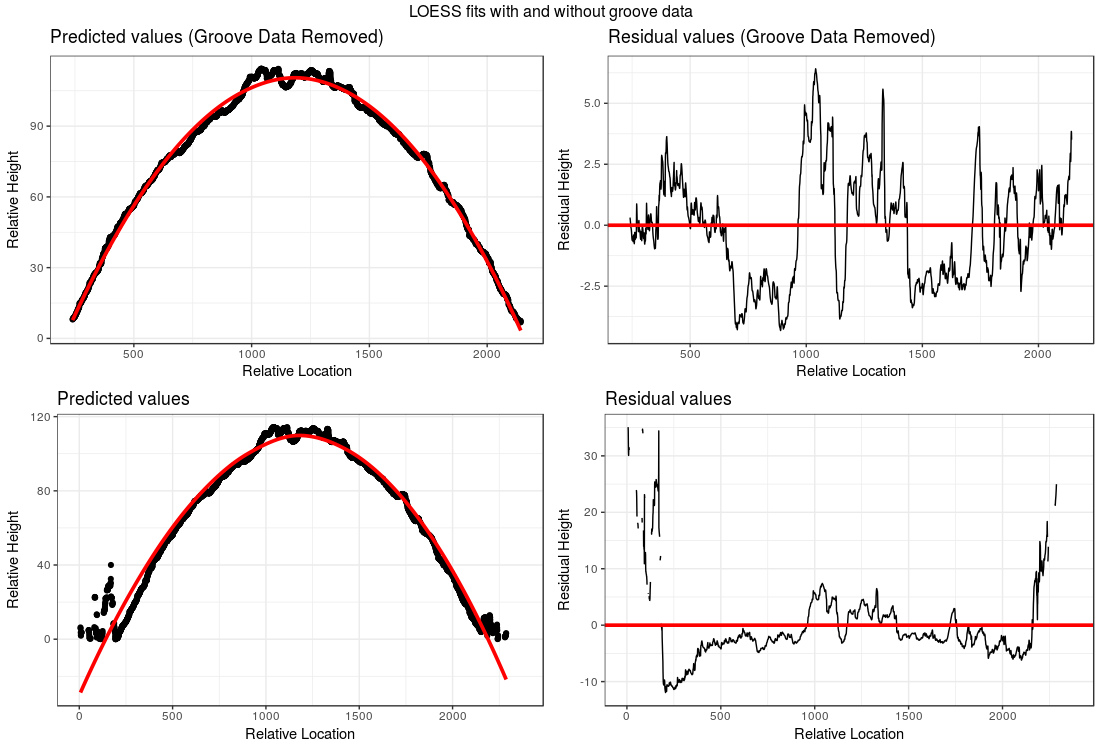
\includegraphics[width=1\linewidth]{images/groove_vs_nogroove} \caption{Example of non-parametric structure removal with groove engraved area data removed (top), compared to non-parametric structure removal with extraneous groove engraved area data (bottom).}\label{fig:grooveremove}
\end{figure}

We implement and compare two methods for fitting the LEA structure.
While the two approaches differ in methodology, they are both rooted in
the ability to mitigate undue influence caused by outlying data.

Once an appropriate fit is obtained, the fitted curve is used to obtain
residual values and determine a good cutoff which separates the two
competing structures.

\subsection{Robust Linear Models}

A natural candidate for a curved structure is a quadratic linear model.
Linear models minimize the vertical squared distance between each data
point and a fitted line. The presence of unusual data near the
boundaries results in a line that is pulled upwards towards GEA data
during the minimization process, as seen in \autoref{lms}. The fit of a
linear model compromises between the LEA and GEA structures, and fails
to fit either structure appropriately.

An alternative approach is a robust linear model which minimizes
absolute deviationsin place of squared deviations. This method of
minimization is less influenced by large outlying values present in the
GEA data. The vast majority of data points are in the LEA structure;
minimization of absolute deviations favors fitting the majority
structure closely and allowing the minority structures on the edges to
have high residual values. Prioritization of the majority structure is
here preferable to the compromise that occurs in traditional linear
models. A striking example of the difference in results from these two
model frameworks is seen in \autoref{lms}.

\begin{figure}
\centering
\includegraphics{writeup_files/figure-latex/lms-1.pdf}
\caption{\label{lms}Example of a quadratic linear model fit and
resulting residuals (top) compared to a robust quadratic linear model
fit and residuals (bottom) for a single profile. The robust model is
able to more effectively capture the curved structure of the LEA without
being influenced by the GEA.}
\end{figure}

The focus on closely fitting majority structure results in residual
values scattered near zero in the LEA and larger, mostly positive
residuals in the GEA zones. Thus, the magnitudes of residuals can serve
as an indicator of membership as LEA data or GEA data. Utilization of a
data-based cutoff value for the magnitude is a practical solution.

The median absolute deviation (MAD), is a robust metric for the spread
of points, similar to the standard deviation. Let \(m\) be the median:\\
\[ MAD(\mathbf{x}) = m(|x_i- m(\mathbf{x})|) \quad \forall\ x_i \in \mathbf{x}.\]
Since we are dealing with unbalanced residual values, the MAD is
preferable to the standard deviation to quantify the spread. Removing
unusually high residual values is effective at removing the GEA data
once the global structure has been fit. Residual values that are
considered unusually high, or outlying, are values that are larger than
4*MAD. Any residual value larger than 4 times the median absolute
deviation value can be seen as a ``large'' residual.

Shoulder location predictions are calculated for each profile in the
following manner:\\

\begin{enumerate}
\item Fit a robust linear model of order 2 (i.e., quadratic) to the averaged profile.   
\item Calculate a residual value for each data point on the profile.  
\item Calculate the median absolute residual (MAD) for the profile.  
\item Remove all data points on the profile whose absolute residual value is greater than 4*MAD.  
\item Identify the range of the remaining x values - these are the predicted shoulder locations for that profile.   
\end{enumerate}

\subsection{Robust LOESS}

Locally weighted regression, known as LOESS, is a non-parametric
approach that is not restricted by the need for perfect quadratic
curvature. This is advantageous when working with bullets, as it is
unrealistic to expect a flawless circular shape to remain after the
bullet has been subjected to the forces of a gun barrel and striae have
been impressed upon it.

LOESS fits many models to small subsets of the data and combines them
into one non-parametric fit of the data, rather than focusing on the
overall structure of the data. This allows for greater flexibility.
However, it also means that LOESS models are affected by GEA structures
in a more unpredictable manner. A model fitted on a subset of data that
mainly falls in the GEA structure can look very different than a model
fit with data from the LEA. This results in a combined prediction that
misrepresents much of the data near one or both boundaries (see
\autoref{loess}).

Robust LOESS utilizes an iterative process focused on re-weighting
\citep[see][]{Cleveland1}. First, an initial LOESS fit is created. This
is followed by a step which gives smaller weights to data points with
high residual values, and a subsequent LOESS fit with new weights
applied. The down-weighting of values with high residual values slowly
reduces the influence of the GEA data. This iterative process results in
a non-parametric fit to the LEA structure that treats GEA data as less
important, which is desirable.

While robust LOESS methods are more flexible than robust linear models,
a model that is accurately fit to the LEA structure results in the same
expected residual structure as with robust linear models: positive and
negative residuals scattered around zero in the LEA zone, and positive,
possibly large residuals in the GEA zones. A similar approach using a
cutoff value can be employed to distinguish between ``large'' residual
values and reasonable ones. Since non-parametric fits offer a closer fit
over a large amount of data, the cutoff for separation will be lower. A
cutoff that performs well on the Hamby set 44 is twice the median
absolute deviation (2*MAD).

\begin{figure}
\centering
\includegraphics{writeup_files/figure-latex/loess-1.pdf}
\caption{\label{loess}Example of a LOESS model fit and residuals (top)
compared to a robust LOESS model fit and residuals (bottom) for a single
profile. The robust model is again able to more effectively capture the
curved structure of the LEA without being influenced by the GEA.}
\end{figure}

Shoulder location predictions are calculated for each profile in the
following manner:

\begin{enumerate}
\item Fit a robust LOESS model with a span of 1 to the averaged profile. This can be fit using the `locfit.robust` function in the `locfit` package in R.
\item Calculate a residual value for each data point on the profile.  
\item Calculate the median absolute deviation (MAD) for the profile.  
\item Remove all data points on the profile whose absolute residual value is greater than 2*MAD.  
\item Identify the range of the remaining Y values - these are the predicted shoulder locations for that profile.   
\end{enumerate}

\section{Results}

In order to assess the accuracy of these predictions, we take a unique
approach. To calculate a quantitative measure for the overall
performance of predictions, we first manually identified ``ground
truth'' shoulder locations.

The numerical comparison of predicted and manually identified locations
can be tricky; distance metrics alone do not suffice to represent the
true character of a prediction's accuracy. For example, a predicted
shoulder location that falls 10 data points away from the manually
identified shoulder location could be caused by noise in the data,
missing data points, or simply the scale of the data. Note that a span
of 10 data points represents only 6.45 microns in physical space.
Alternatively, a distance of 10 points could indeed be part of the
groove engraved area, and thus being incorrectly identified could
potentially cause problems in subsequent analyses.

A more suitable measure is to investigate the residual values resulting
from the robust LOESS model that fall in the range spanned by the
predicted and manually identified shoulder location. This method
penalizes shoulder location predictions that are too far out to the side
and leave GEA data in the main structure.

Because the robust LOESS most reliably approximates the curved shape of
the bullet land due to its flexibility, we want to use residual values
resulting from that model to assess final performance of all methods.
Residual values from the GEA will not necessarily be uniformly large,
but are expected to be positive as their structure and the modeling
technique dictate that they would fall above the fitted line from robust
LOESS.

With positive residuals in the GEA, even a 10-point difference can
quickly add to a large residual sum. However, a 10-point difference
within the land engraved area will be balanced out by the presence of
both positive and negative residual values and remain closer to zero.

For this reason, gathering the sum of residuals between the predicted
location and the manually identified location is appropriate. This
residual sum is referred to as an ``inaccuracy score'' for which higher
values indicate a higher level of inaccuracy. An inaccuracy score was
calculated separately for the left hand side and right hand side
predictions for each profile in the data set. This was calculated for
the Robust Linear Model and Robust LOESS methods, as well as the
Rollapply method suggested in \citet{Hare1}.

Of interest are the distributions of these inaccuracy scores across all
208 lands used in the study (see \autoref{results1}). A distribution
that has a smaller spread and is close to zero is ideal; this suggests
many of the predicted shoulder locations are very close to the manually
identified locations, and predictions are removing many of the outlying
GEA points. A distribution with a wider spread or many high, outlying
inaccuracy scores suggests a greater degree of uncertainty and
inaccuracy for a particular method.

\begin{figure}
\centering
\includegraphics{writeup_files/figure-latex/results1-1.pdf}
\caption{\label{results1}Distribution of inaccuracy scores for data
smoothing method, robust linear model method, and robust LOESS method,
separated by left and right shoulder locations. A tight distribution
with few high values indicates good performance across the LEAs in the
data set.}
\end{figure}

The raw distributions can be difficult to visually compare, so another
way to inspect the results is to place inaccuracy scores into
categories: satisfactory, borderline, unsatisfactory. Scores under 100
are satisfactory, scores between 100 and 1000 are borderline, and scores
above 1000 are unsatisfactory (see \autoref{results2}). Unsatisfactory
cases are the most likely to cause mistakes in subsequent analyses.

It is important to note that different results are expected for the left
and right shoulder locations. Within Hamby set 44, almost all scans have
a well-defined left groove. Left here is defined as visually left on the
scan; this is the side the scan begins on, so a well-defined distinction
between GEA and LEA is expected. Often, a less clear distinction is seen
on the right side of the scan, with sometimes no apparent shoulder
location visible. For this reason it is preferable to separate the left
and right for visual inspection of results; a method may excel on one
side but fall short on another.

\begin{figure}
\centering
\includegraphics{writeup_files/figure-latex/results2-1.pdf}
\caption{\label{results2}Distribution of inaccuracy scores for data
smoothing method, robust linear model method, and robust LOESS method,
separated by left and righth shoulder locations. Inaccuracy scores are
placed into three categories: less than 100 microns (satisfactory),
between 100 and 1000 microns, and greater than 1000 microns. A larger
proportion of inaccuracy scores under 100 microns indicates good
performance across LEAs in the data set.}
\end{figure}

\section{Conclusions}

Both the robust linear model and robust LOESS approaches outperform
currently implemented solutions based on data smoothers. Of the two, the
robust LOESS approach clearly outperforms the robust linear model. This
hierarchy of performance is well within expectation given the strength
of robust approaches in general as well as the flexibility of LOESS
applied to this data type. Robust LOESS also readily handles variation
introduced in the process of translating the physical bullet into a 3D
object. If there is too much variability in how the bullet is placed
relative to the plane of reference on the microscope, profiles can have
tilted shapes relative to the x-axis which a quadratic linear model
would fail to address. In these situations, LOESS excels.

While the cutoff values presented work well on Hamby set 44, additional
validation will need to be implemented on a variety of bullet types.
Depth of striae, physical size of bullet due to caliber, and
non-traditional rifling techniques may require alterations to this
cutoff value. In addition, a study of the effect of implementing a
robust LOESS data pre-processing strategy on overall automated
image-analysis methods will need to be addressed. Due to increased
accuracy of predicted shoulder locations, the authors expect an increase
in accuracy in bullet matching algorithms. However, this will need to be
validated on a variety of data sets prior to implementation without
human intervention in the automated process.

\section{References}

\bibliography{bibliography.bib}


\end{document}
